% Chapter 6

\chapter{RESULTS AND DISCUSSION} % Write in your own chapter title

\section{Output Obtained in Various Stages}
\subsection{Blockchain Network Setup}
To implement a blockchain we have to setup network by creating
Orderer and peers. Following figures explain the implementation
of blockchain (6.1 to 6.4)
\begin{figure}[htb!]
  \centering
 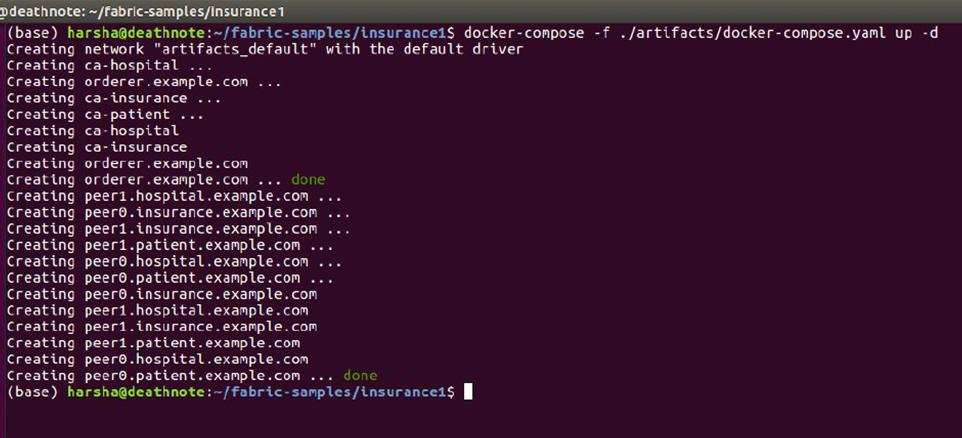
\includegraphics[width = 15cm, height = 5cm] {Figures/docker.jpg}
  \caption{Docker Creation}
  \label{StH}	
\end{figure}

\begin{figure}[htb!]
  \centering
 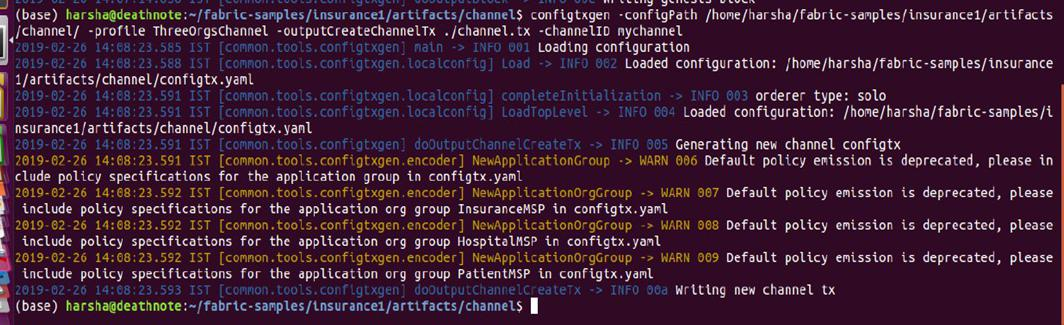
\includegraphics[width = 15cm, height = 5cm] {Figures/channel.jpg}
  \caption{Channel Creation}
  \label{StH}	
\end{figure}

\begin{figure}[htb!]
  \centering
 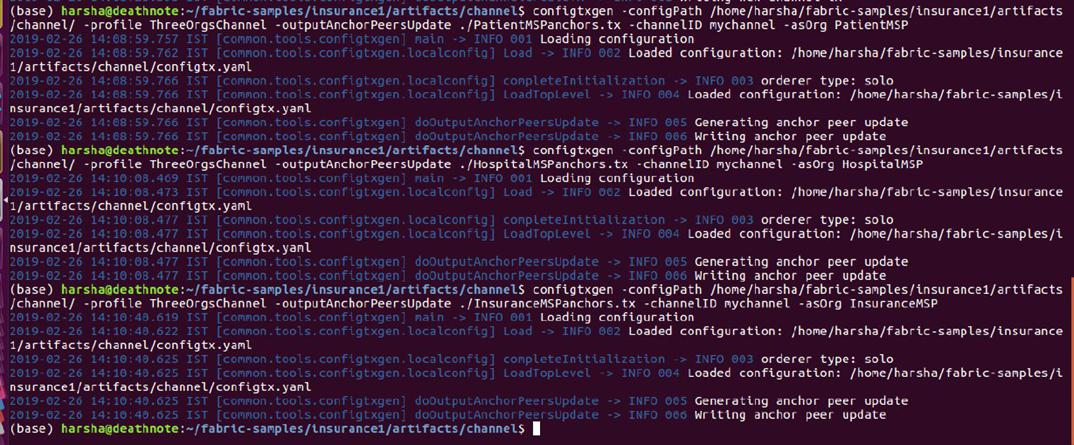
\includegraphics[width = 15cm, height = 6cm] {Figures/peer.jpg}
  \caption{Peer Creation}
  \label{StH}	
\end{figure}

\begin{figure}[htb!]
  \centering
 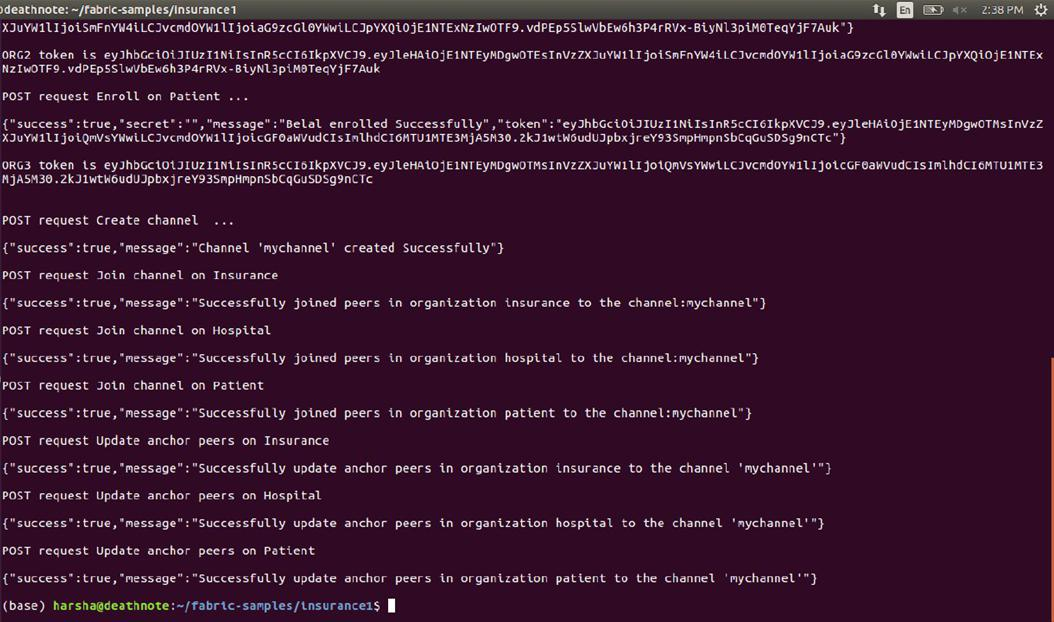
\includegraphics[width = 15cm, height = 8cm] {Figures/join.jpg}
  \caption{Peer Joining}
  \label{StH}	
\end{figure}

\subsection{Genesis Block}
The genesis block for bootstrapping the blockchain application is created using configtxgen tool which is an inbuilt tool with Hyper ledger. This tool takes an input file configtx.yaml and outputs the binary file which should be used when creating initial setup for blockchain as shown in Figure 6.5
\begin{figure}[htb!]
  \centering
 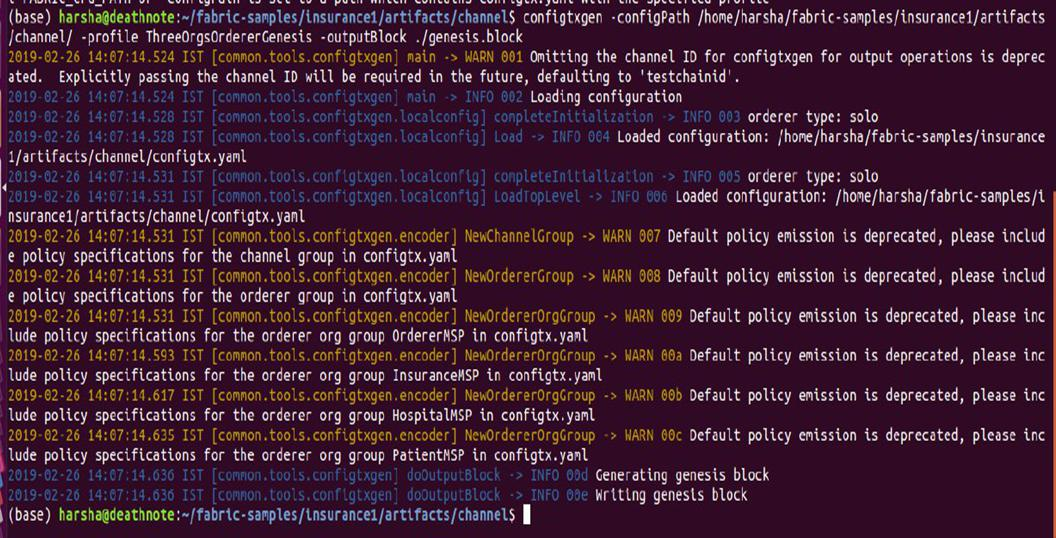
\includegraphics[width = 15cm, height = 5cm] {Figures/genesis.jpg}
  \caption{Genesis Block Creation}
  \label{StH}	
\end{figure}

\subsection{Smart Contract}
It takes the Bill ID and Bill amount as input. Smart Contracts automatically claims the patient bill amount whose insurance amount must be less than the insurance limit. And if the insurance amount is less than or equal to the insurance limit the data is sent to the encrypted phase if not it is discarded as shown in Figure 6.6
\begin{figure}[htb!]
  \centering
 \includegraphics[width = 15cm, height = 5cm] {Figures/smart.jpg}
  \caption{Smart Contract}
  \label{StH}	
\end{figure}

\subsection{Private Key Encryption}
It takes the patient treatment details as the input and encrypts the data using RSA Algorithms and produces the encrypted data as shown in 6.7
\begin{figure}[htb!]
  \centering
 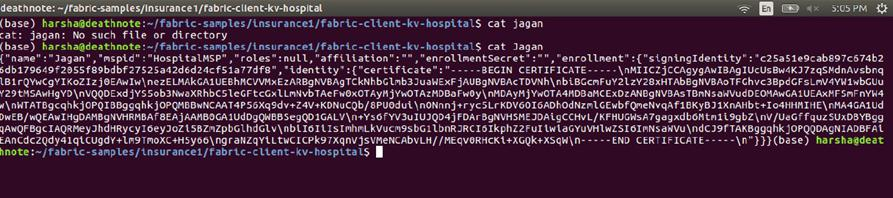
\includegraphics[width = 15cm, height = 3cm] {Figures/private.jpg}
  \caption{Private Key Enc}
  \label{StH}	
\end{figure}

\subsection{Hashing}
It takes the block containing the block header and transaction header as the input and hashes the data in the block using SHA-256 algorithm. This is shown in figure 6.9
\begin{figure}[htb!]
  \centering
 \includegraphics[width = 15cm, height = 6cm] {Figures/hash.jpg}
  \caption{Hashing}
  \label{StH}	
\end{figure}

\subsection{Preprocessing}
It takes the encrypted data as input and checks all the necessary data to instantiate a claim that has been uploaded or not and produces the block containing the block header and transaction header. This is shown in figure 6.9
\begin{figure}[htb!]
  \centering
 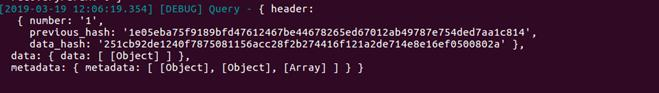
\includegraphics[width = 15cm, height = 3cm] {Figures/pe.jpg}
  \caption{Preprocessing}
  \label{StH}	
\end{figure}

\subsection{Tamper Proofness}
When the unknown party tries to access the permissioned
blockchain then it will show error and won’t allow him/her to access
the data. This is shown in figure 6.10
\begin{figure}[htb!]
  \centering
 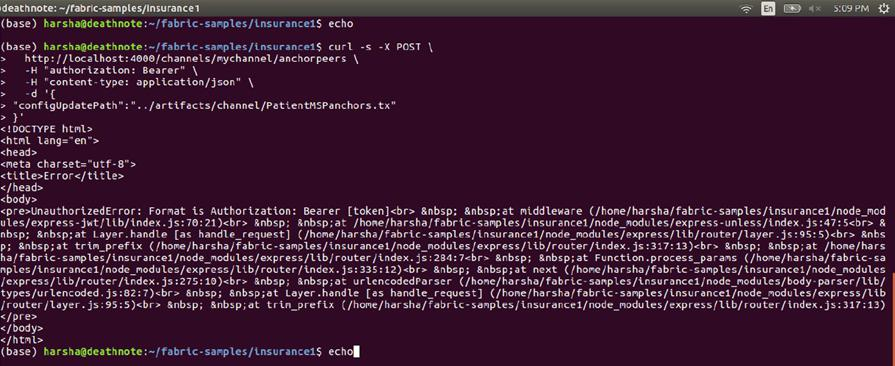
\includegraphics[width = 15cm, height = 6cm] {Figures/tamper.jpg}
  \caption{Tamper Proofness}
  \label{StH}	
\end{figure}

\section{Performance Evaluation}
\subsection{Throughput}
Throughput will be measured as the number of successful transactions
per second. A workload can be configured with multiple clients and
threads per clients to saturate the blockchain throughput.
\[Throughput=\frac{Number of successful Transactions}{Total amount of time}\]
\begin{figure}[htb!]
  \centering
 \includegraphics[width = 15cm, height = 6cm] {Figures/throughput.jpg}
  \caption{Throughput}
  \label{StH}	
\end{figure}